\subsection{Instrumentation}
\label{subsec:hardware}
Fig.~\ref{fig:testbed} shows the testbed. Four LEDs are mounted on the ceiling, 3.0~m above the floor and facing down. Each is intensity-modulated by its own sinusoidal tone, at 300, 500, 700 and 900~kHz, so that the four contributions are separated in frequency at the receiver. The method uses a single LED: the 500~kHz LED is the positioning transmitter of this work. The other three are recorded simultaneously only to repeat the evaluation with different LEDs, each used alone as an independent single-LED system (Section~\ref{subsec:res-leds}).
% AUTHOR: add the LED model, the LED drivers (bias and modulation depth) and the signal generators.

The receiver is a Thorlabs PDA100A2 amplified silicon photodetector (active area 75.4~mm$^2$, gain set to 20~dB), AC-coupled to a Keysight MSO-X 4154A oscilloscope. It is reoriented by a Thorlabs MTRS motorized stage, whose rotation axis is vertical; the small tilt of the stage is kept at zero, and the inclination of the PD is provided by a 3D-printed adapter with $t=15^\circ$ (Section~\ref{subsec:design}), as shown in Fig.~\ref{fig:receiver}. At stage angle $\theta_i$, the normal of the PD is:
\begin{equation}
 \vect n_i=\left[\sin t\sin(\theta_i-\theta_0),\ \sin t\cos(\theta_i-\theta_0),\ \cos t\right]\trans,
 \label{eq:normal}
\end{equation}
where $\theta_0$ is the stage angle at which the PD tilts towards $+Y$; the stage turns at $1.5^\circ$/s. The angles are commanded as $\theta_i=(65^\circ+360^\circ k/K)\bmod360^\circ$, $k=0,\ldots,K-1$, visited in increasing order, and the encoder readings are used in the estimator. The stage and PD are carried by an igus DLE-RG-0012-BLDC Cartesian gantry, which positions the receiver over $1.4\times1.4$~m horizontally and provides the ground truth.

At every orientation, after a settling time of 1~s, the oscilloscope records 100~ms of the PD output at 10~MSa/s ($N=10^6$ samples) in digitizer mode, and the record is transferred over the local network. The RSS of each LED is the projection~\eqref{eq:lockin} at its nominal frequency, with a resolution of 10~Hz. The raw record of every measurement is kept, which allows shorter windows to be evaluated afterwards (Section~\ref{subsec:res-window}). The tones differ from their nominal frequencies by about 1.1~ppm ($-0.36$ to $+0.96$~Hz, measured from their phase drift along the records), so the projection of a 100-ms record at the nominal frequency reads 0.2--1.5\,\% low depending on the tone (0.5\,\% at 500~kHz). This factor is common to calibration and positioning when both use the same window, and is then absorbed by $A$. The raw PD signal is dominated by the 100~Hz flicker of the room lights (about 120~mV rms against LED tones of 1--21~mV); the projection rejects it, but the flicker sets the vertical scale of the oscilloscope.

An in-house acquisition program coordinates the gantry, the stage and the oscilloscope, stores the commanded and measured poses, the RSS and the raw records, and resumes interrupted campaigns automatically. The same estimation code runs in a real-time demonstrator that moves the receiver to a position, acquires the $K$ orientations and displays the estimate; it produced the blind test of Section~\ref{subsec:res-blind}.

\begin{figure}[!t]
 \centering
 % PHOTO TO BE TAKEN BY THE AUTHOR: overall view of the testbed (ceiling LEDs, gantry, stage with the PD, oscilloscope),
 % ideally with the X, Y, Z axes of the global frame overlaid.
 \figplaceholder{4.8cm}{Photograph of the testbed: four ceiling LEDs, Cartesian gantry carrying the rotation stage and the PD, and oscilloscope; global axes $X$, $Y$ (gantry) and $Z$ (up) overlaid.}
 \caption{Experimental testbed. The gantry moves the receiver over $1.4\times1.4$~m; the LEDs are 3.0~m above the floor.}
 \label{fig:testbed}
\end{figure}

\begin{figure}[!t]
 \centering
 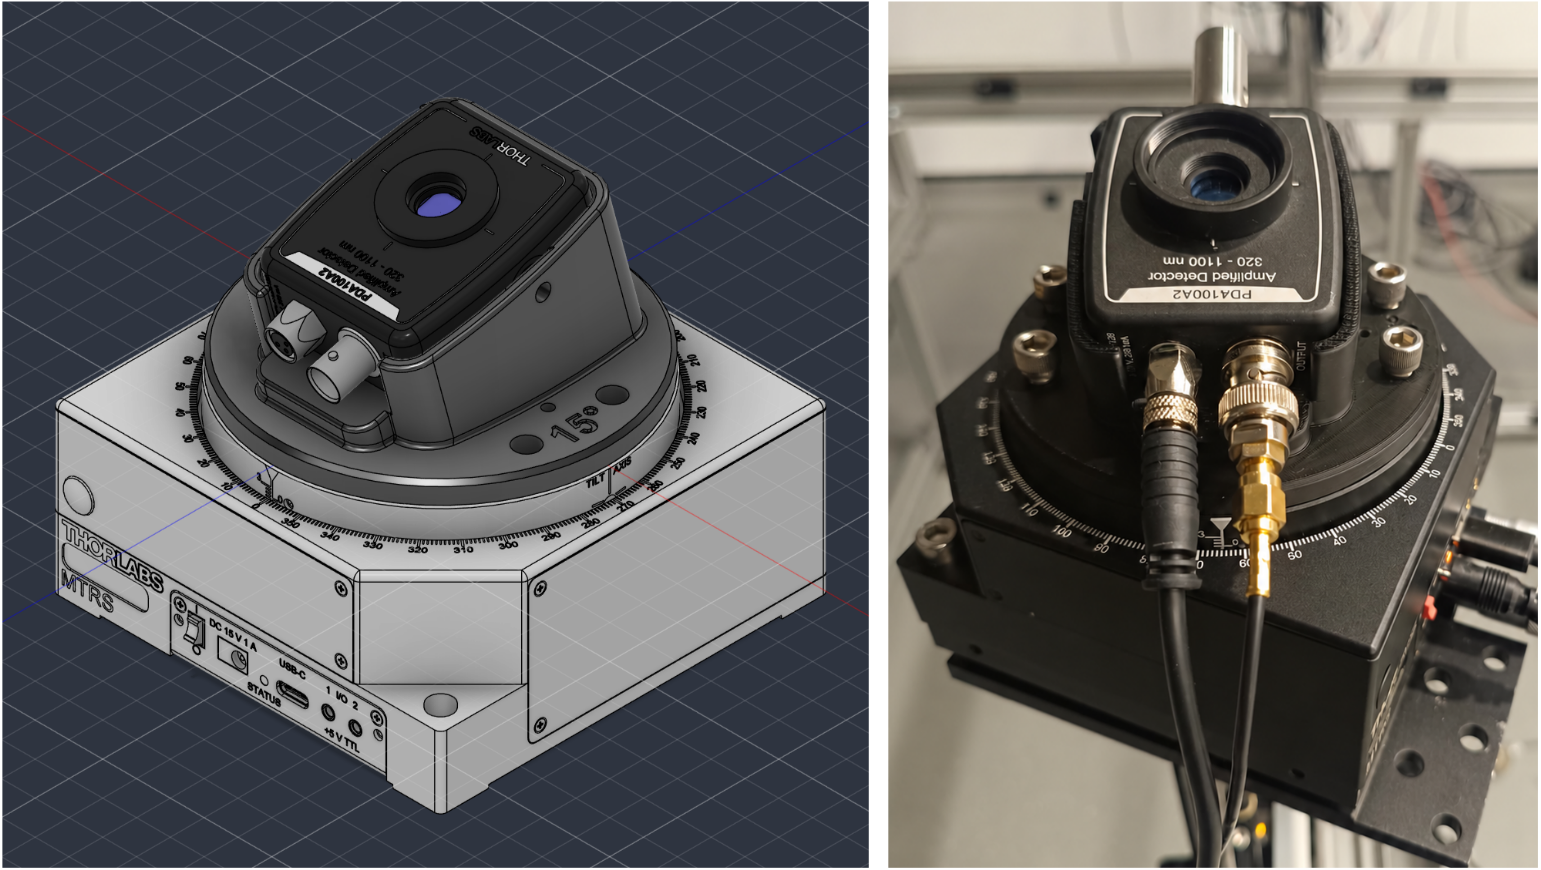
\includegraphics[width=\linewidth]{fig_inkscape/fig_PD.png}
 %\figplaceholder{4.2cm}{PD on the rotation stage with the $15^\circ$ adapter (photograph or CAD), and the normal convention of~\eqref{eq:normal}: stage angle $\theta_i$, zero $\theta_0$ (tilt towards $+Y$), tilt $t$ and elevation $e$ of the PD center above the gantry carriage.}
 \caption{Receiver assembly. The adapter tilts the PD by $t=15^\circ$ with respect to the vertical rotation axis of the stage, so that turning the stage sweeps the PD normal over a cone.}
 \label{fig:receiver}
\end{figure}

\subsection{Reference Frame and Ground Truth}
\label{subsec:groundtruth}
Positions are expressed in the gantry axes $X$ and $Y$ and in the height $Z$ above the floor. The center of the PD is at height $Z=0.858~\mathrm m+z+e$, where $z$ is the vertical coordinate of the gantry, 0.858~m the height of the gantry carriage at $z=0$ (measured with a tape, 1.038~m at $z=180$~mm) and $e=96.96$~mm the elevation of the PD center above the carriage, taken from the CAD model of the stage and adapter. The rotation axis of the stage passes through the PD center, which therefore does not move during a reorientation. The LED plane, at 3.000~m, was measured with a tape; the horizontal position of the LED was not surveyed and is obtained from the calibration (Table~\ref{tab:parameters}).
% AUTHOR: state the resolution/uncertainty of the tape measurements and the positioning repeatability of the gantry.

\subsection{Datasets}
\label{subsec:datasets}
Three datasets were acquired with the same instrumentation (Table~\ref{tab:datasets}).

\emph{D1, calibration and environment.} The PD, on a $0^\circ$ adapter and facing up ($K=1$), scanned a $141\times141$ grid with 10~mm spacing over the whole $1.4\times1.4$~m area, at a PD height of 1.135~m, i.e., $h=1.865$~m below the LED plane. The 19\,881 records contain the four LEDs and serve two purposes: they characterize the radiation patterns of the LEDs (Section~\ref{subsec:res-env}), and they calibrate the LED model through~\eqref{eq:led-calibration}. The values of Table~\ref{tab:parameters} were obtained from the first 14\,294 points (the region within 1.16~m of the LED); a joint fit over the whole map gives the same accuracy (Section~\ref{subsec:res-budget}).

\emph{D2, regular grid.} With the $15^\circ$ adapter, the receiver visited a $5\times5$ horizontal grid ($X,Y$ from 0.1 to 1.3~m, step 0.3~m) at five heights ($Z=0.955$, 1.015, 1.075, 1.135 and 1.315~m), i.e., 125 positions, with $K=10$ orientations each ($\theta_i=65^\circ+36^\circ k$).

\emph{D3, blind random test.} The real-time demonstrator drew random positions uniformly in $X,Y\in[0.1,1.3]$~m and $Z\in[0.955,1.315]$~m and estimated each one live with $K=5$ ($\theta_i=65^\circ+72^\circ k$), using the parameters of Table~\ref{tab:parameters} fixed beforehand. The test contains 131 positions acquired in two sessions. A further 44 positions of the first session, acquired after the tilt axis of the stage moved by itself, are excluded and analyzed in Section~\ref{subsec:res-integrity}; a later dense-grid campaign affected by slippage of the rotation stage was likewise discarded.

\begin{table}[!t]
 \centering
 \caption{Datasets}
 \label{tab:datasets}
 \footnotesize
 \setlength{\tabcolsep}{3pt}
 \begin{tabular}{@{}lccc@{}}
 \toprule
 & D1 calibration & D2 grid & D3 blind test\\
 \midrule
 Positions & 19\,881 & 125 & 131\\
 Layout & $141\times141$, 10~mm & $5\times5\times5$ & Random\\
 PD height (m) & 1.135 & 0.955--1.315 & 0.955--1.307\\
 Adapter tilt & $0^\circ$ & $15^\circ$ & $15^\circ$\\
 Orientations $K$ & 1 & 10 & 5\\
 Records (100~ms) & 19\,881 & 1\,250 & 655\\
 Use & LED model & Evaluation & Blind test\\
 \bottomrule
 \end{tabular}
\end{table}

\subsection{Protocol and Metrics}
\label{subsec:protocol}
The LED parameters come only from D1. The angular zero $\theta_0$ of the stage is a property of the receiver assembly and is calibrated with the shape test~\eqref{eq:shape} at known positions. When D2 is evaluated, the zero used at each height is fitted on the other four heights (leave-one-height-out); the five values range from $66.41^\circ$ to $66.54^\circ$, and the fit over all of D2, $66.5^\circ$, is the value frozen for D3. No parameter is adjusted on D3. Unless stated otherwise, positions are estimated with the SQ response and the NLS estimator~\eqref{eq:nls}--\eqref{eq:range}.

The accuracy is reported by the 3D error $\norm{\hat{\vect r}-\vect r}$, its horizontal component, the signed vertical error (positive when the estimate is above the true position) and the angle between $\hat{\vect u}$ and the true direction; statistics are the mean, median, root-mean-square error (RMSE), 90th percentile (P90) and maximum, and estimator failures are counted separately. To study the number of orientations without new acquisitions, the $K=10$ angles of D2 are subsampled into near-uniform subsets of $K$ angles, with indices $\operatorname{round}(10j/K)$, $j=0,\ldots,K-1$, and all their rotations.
